\chapter{Spettroscopia NMR}

L'NMR è una tecnica spettroscopica, che permette di vedere transizioni di spin. È una tecnica non distruttiva,
quindi è preferenziale rispetto alla massa. Non è invasiva. È una
tecnica veloce: una analisi dura da minuti per il protone a diverse ore per il carbonio-13.

Si possono studiare processi dinamici; da informazioni anche
quantitative. Questo è dato dal fatto che si possano fare molti tipi di
esperimenti di NMR.

\fullpicture*{4_001}{Spettri NMR monodimensionale e bidimensionale o di correlazione}

Nell'NMR, si vedono i nuclei che hanno spin. Se I è diverso da 0, non si
possono analizzare all'NMR. Si vedono meglio i nuclei con I = 1/2.

Questo si vede negli spettri di \ap{1}H e di \ap{13}C, dove entrambi hanno I=1/2.

\marginpicture*{4_002}{Nucleo magnetico}

Quando si fa un esperimento di NMR si immergono i nuclei in un campo
magnetico. Le direzioni dei momenti magnetici si allineano, e visto che
è un numero quantico, si hanno delle direzioni quantizzate.
In nuclei si orientano nello stesso verso del campo, o nel verso opposto del
campo.

\fullpicture*{4_003}{Allinuamento dei nuclei}

Il numero quantico in questione è $m$. Questi sono gli stati di spin
dell'NMR. Questo è possibile perché bisogna vedere una transizione; si
hanno due stati di spin e questo provoca che si possa fare una
transizione tra queste due. È possibile che avvenga una transizione
La differenza di energia è
\[
\Delta E = E_\beta - E_\alpha = \gamma \hbar B_0
\]

All'inizio, gli stati di spin sono tutti uguali. Dopo il campo magnetico
gli stati si separano. La distribuzione di questi due stati segue la
distribuzione di Boltzmann.

Lo stato superiore è popolato, quindi è un problema, perché la tecnica
di base è poco sensibile. Non si ha un salto visibile.

Tanto maggiore è il campo magnetico e tanto maggiore è la separazione. A
parità di campo magnetico, nuclei che hanno \(\gamma\) elevato aumentano
la separazione.

Nell'NMR il nucleo risuona; quando il nucleo viene colpito da una radiazione di uguale energia alla separazione, il nucleo risuona. Questa
risonanza ha una frequenza ben definita. Questa frequenza si chiama frequenza di Larmor.

Per definire lo strumento NMR si usa la frequenza di Larmor (200 MHZ, etc).
La differenza di energia tra i due stati di spin è sempre piccola, anche se il campo è molto intenso.

La costante giromagnetica per il protone è molto elevata, mentre per il \ap{13}C non
è così elevata. Questo, unito al fatto che il \ce{^{13}C} non è molto abbondante fà si che l'NMR per questo nucleo necessiti di più tempo.

\begin{figure}[H]
  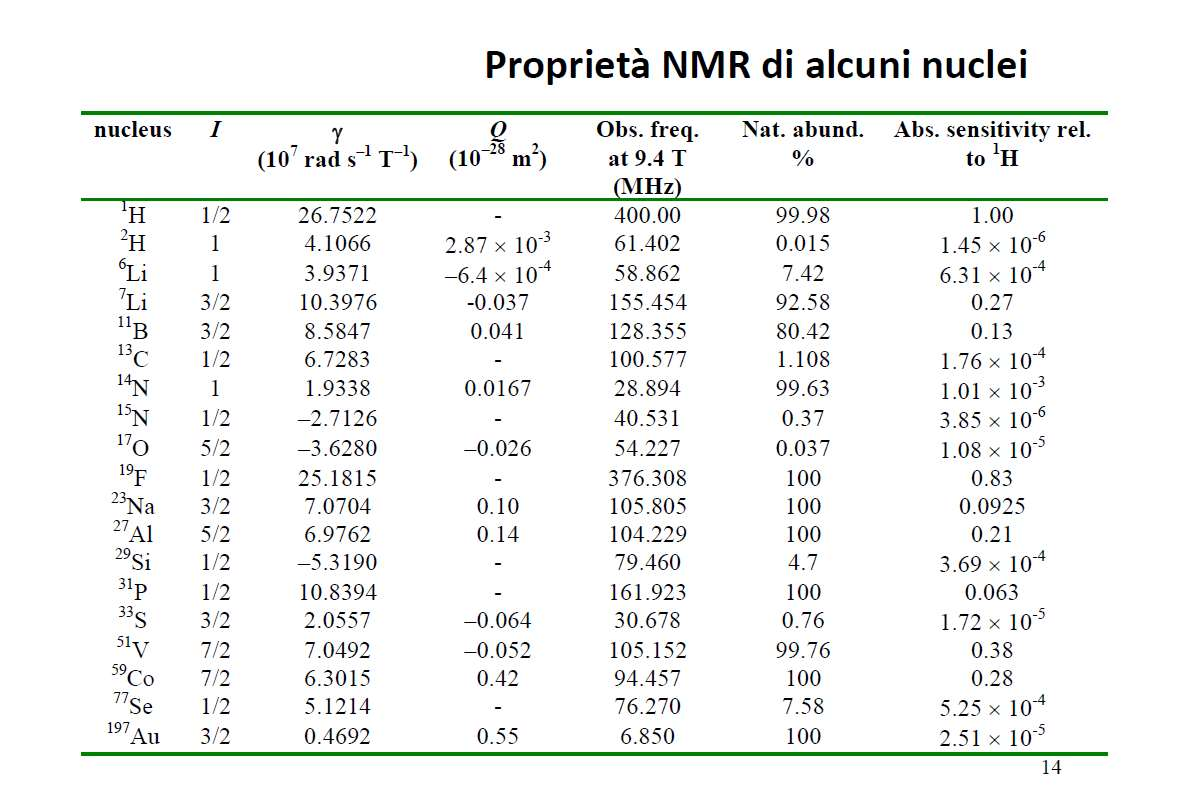
\includegraphics[width=\textwidth]{4_005}
\end{figure}

\marginbox*{
  È importante che il magnete sia schermato. In modo che il campo magnetico non arrivi all'utente. Gli strumenti vecchi sono rinchiusi in una stanza, dove non si può accedere.
}

Per uno stesso campo magnetico, si possono  differenziare nuclei di elementi differenti, o anche nuclei uguali, con diversi intorni chimici.

I nuclei non sono isolati, ma hanno un intorno elettronico. La nuvola di
elettroni scherma il nucleo. Più è grande e meno il campo magnetico
riesce a passare.
Ogni nucleo quindi risente di un campo magnetico effettivo diverso.

Il campo magnetico effettivo è sempre minore del campo magnetico
applicato. I nuclei non equivalenti hanno frequenze di risonanza
diverse. Quindi si hanno segnali diversi per ogni protone non-equivalente.

I gruppi elettron-attrattori diminuiscono la densità elettronica intorno
al nucleo, cioè il nucleo è meno schermato e sente di più un campo
magnetico esterno. Di conseguenza il nucleo avrà una maggiore frequenza
di risonanza.
Un gruppo elettron-donatore, avrà l'effetto contrario.
Questo è il principio che spiega tutti gli spostamenti dei segnali nell'NMR.

\fullpicture{4_006}{Frequenza di Larmor vs elettronegatività}{fig:Larmor}

Nel grafico \ref{fig:Larmor} si vede questo principio. Maggiore è
l'elettronegatività, più aumenta la frequenza di Larmor.

\paragraph{Segnali}

Nello spettro NMR ci possono essere alcuni segnali sovrapposti; questa non è una situazione ottimale, in quanto è difficile associare un segnale ad un atomo.
Se però i due segnali sono distanti, è più facile associare un segnale

Per comparare diversi strumenti NMR, si usa la \vdirg{scala dello spostamento chimico}. Questa scala fa riferimento
alla frequenza del protone di una molecola di riferimento e consente di comaparare i dati.
Si usa il tetrametilsilano. Questa molecola possiede dodici protoni quindi il segnale prodotto è molto intenso. La misura è data in $ppm$
(parti per milione), in quanto è indipendente dal campo magnetico $B_0$.
\[
  \delta = \frac{\nu - \nu_{\text{ref}}}{\nu_{\text{ref}}} \times 10^6 \qquad \delta = \frac{\nu - \nu_{\text{ref}}}{\nu_{\text{strumento}}} \times 10^6
\]

In questo modo si può guardare lo spostamento del segnale e si può
ricostruire la struttura della molecola.

\paragraph{Risoluzione}

Uno strumento che lavora a frequenza più alta ha più risoluzione. Un ppm
non ha lo stesso valore, ma si basa sul campo magnetico dello strumento.



Il segnale di riferimento viene posto zero e viene messo a destra dello spettro.
Si registra lo spettro tra 0 e 14 ppm, per \ce{^{1}H} NMR

\section{Informazione strutturale}

L'NMR dà informazioni strutturali. Si vede che il numero di segnali dà il numero di protoni presenti nella molecola.

La posizione del segnale dà informazione qualitativa, che consente di associare il segnale ad un ben specifico protone. Mentre, l'area ad di sotto del segnale fornisce informazione quantitativa,
ovvero riesce a determinare il numero di protoni che danno quel segnale.

Se due protoni equivalenti avranno la stessa frequenza di risonanza ed avranno lo stesso spostamento chimico. Questo ragionamento non può
essere fatto al contrario; se due protoni sono diversi, potrebbero anche
avere lo stesso segnale.
Due protoni sono equivalenti se c'è una simmetria molecolare o se è
possibile lo scambio chimico.

\subsection{Simmetria}

Per vedere se una molecola è simmetrica, bisogna cercare un operazione di simmetria che consenta di avere una molecola sovrapponibile.

\halfpicture*{4_007}{Elementi di simmetri di alcune molecole}

Si vede che nell'etilene esistono due piani di simmetria. Tutti i protoni del doppio legame sono equivalenti.

Se si sostituiscono due idrogeni con due metili, si possono avere un piano di simmetria, se la molecola è l'alchene è cis, oppure una rotazione di 180°, se la molecola è trans.

\marginpicture*{4_009}{Nel gruppo metila avviene una rapida rotazione intorno al legame. In una conformazione statica, i tre protoni metilici sarebbero distinguibili, la la rapida rotazione li rende equivalenti. Il chemical shift osservato è quello medio. Il sistema è A\ped{3}}

Nel metile, i tre protoni sono sempre equivalenti. La
rotazione del legame C-C è molto veloce. Non importa se la molecola ha
un centro chirale o altro, questa rotazione è sempre consentita; i
protoni sono sempre equivalenti.

\begin{figure}[H]
  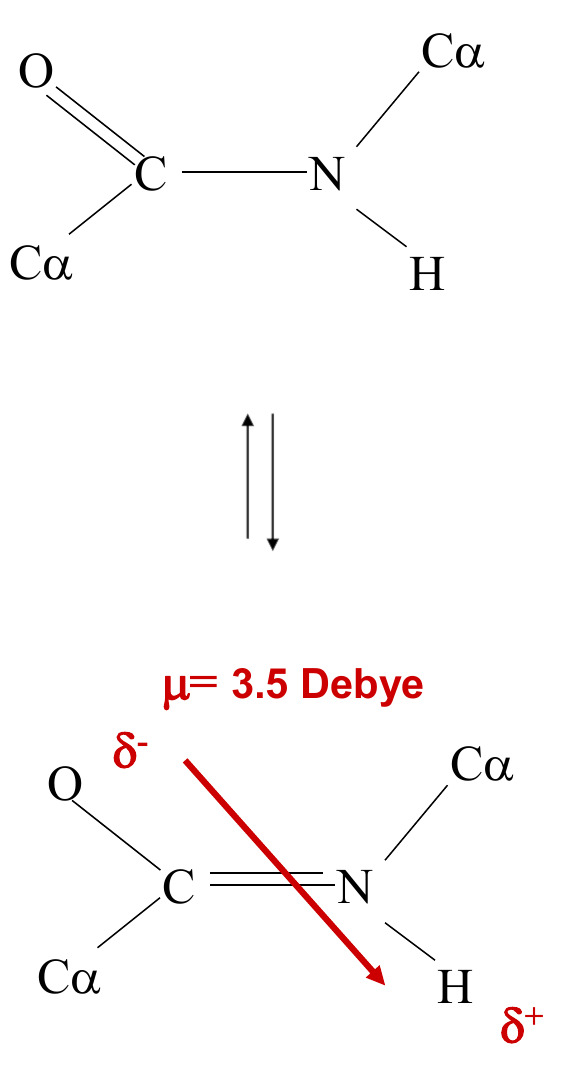
\includegraphics[width=0.6\textwidth]{4_008}
\end{figure}

Nel metilene, si ha ancora la rotazione veloce intorno al legame sigma. La rotazione
darà diverse conformazioni che scambiano velocemente.

\marginpicture*{4_010}{La rapida rotazione attorno al legame \ce{C-C} rende i due idrogeni indistinguibili, a patto che il gruppo metilenico sia adiacente ad un gruppo non chirale. Il sistema è A\ped{2}X\ped{2}}

I protoni a e b sono equivalenti, si ha lo stesso intorno chimico 

\marginpicture*{4_011}{I protono metilenici non sono equivalenti per simmetria e non lo diventano nemmeno per rotazione attorno al legame C-C. Sono diasterotopici}

Se si ha un centro chirale adiacente al metilene, le conformazioni sono
tutte diverse. I due protoni non sono equivalenti.
Questo succede sempre se si ha un gruppo metilenico vicino ad un gruppo
chirale. Si avranno quindi due segnali nellos spettro NMR.

Per capire se i due protoni sono equivalenti si utilizza la sostituzione
(o marcatura). Si vanno a sostituire i due protoni con due gruppi
diversi A e B.

Si può determinare la topicità dei protoni
\begin{itemize}
  \item \textit{Omotopici:} i due protoni sono equivalenti (identici)
  \item \textit{Enantiotopici:} i due protoni sono enantiomerici se la sostituzione produce un enantiomero
  \item \textit{Diastereotopici:} se la sostituzione dei due protoni produce un diastereoisomero.
\end{itemize}

Nel primo caso, la sostituzione dei due protoni produce la stessa
molecola; sono omotopici.
Nel secondo caso, la sostituzione di due protoni produce due enantiomeri
diversi; quindi i due protoni sono enantiotopici. In questo caso cambia
il potere ottico rotatorio. In questa molecola c'è anche una simmetria
piano di inversione.
Nel terzo caso, i due protoni sono diastereotopici; la loro sostituzione
crea due diastereoisomeri.

\subsubsection{Casi particolari}

Se il metilene non è contiguo ad un centro chirale allora i protoni sono
molto simili; la differenza in chemical shift è molto bassa (0.01 ppm). I
protoni sono comunque diastereotopici.

Più vicini sono i protoni al centro chirale e più c'è la separazione a
livello di chemical-shift. La differenza deve essere maggiore di quella
in figura \ref{fig:ProtoniMetilenici}.

\halfpicture{4_013}{Chemical shift per due protoni metilenici}{fig:ProtoniMetilenici}

Altri casi particolari, sono i composti meso.
Un altro esempio è il glicerolo, che è achirale, però i due protoni del carbonio al
centro danno segnali differenti.

\begin{figure}
  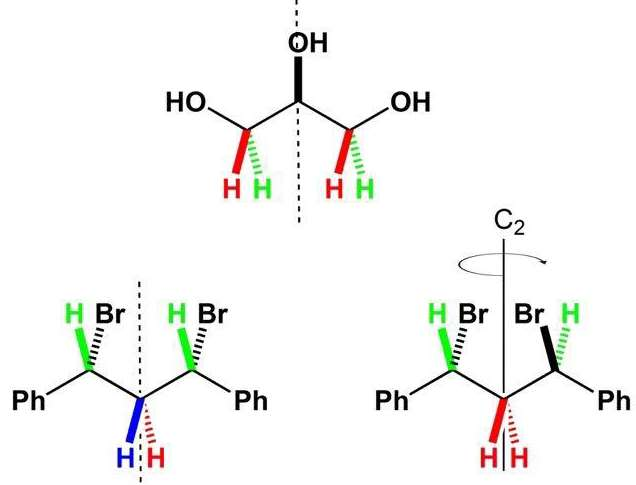
\includegraphics[width=0.5\textwidth]{4_014}
\end{figure}

Per vedere la topicità di due o più atomi, bisogna sostituire alternativamente questi atomi con uno differente e vedere che risultato produce. Infatti, se si crea un centro chirale, i due protoni sono enantiotopici. Se però è già presente un centro chirale nella molecola, allora i due protoni sono diasterotopici. Se invece la sostituzione produce gli isomeri cis e trans, allora sono eterotopici. Se, infine, la molecola ottenuta è la stessa, allora i due atomi sono omotopici.


\section{Chemical shift dei protoni}

\begin{itemize}
\item
  I protoni che danno segnali più bassi, ovvero sono più schermati, sono degli
  alcani che vanno da 0 a 4 ppm
\item
  I protoni del doppio legame li susseguono
\item
  I protoni degli aromatici li susseguono
\item
  E infine ci sono dei protoni dei carbonili
\end{itemize}

\begin{figure}[H]
  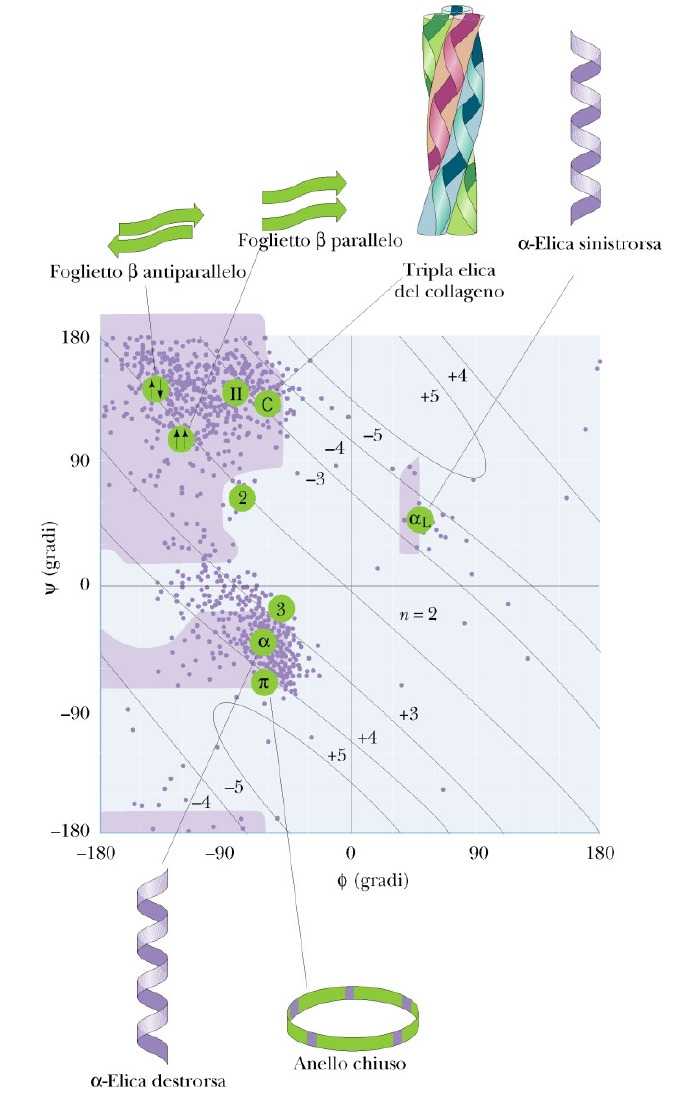
\includegraphics[width=\textwidth]{4_015}
  \caption*{La scala dei chemical shift caria da 0 a 10 ppm per la maggioranza dei protoni. Per convenzione, il TMS ha \delta = 0 e lo spettro NMR è riportato con i chemical shift cerso sinistra.}
\end{figure}

Gli alchini hanno i protoni in mezzo alla regione degli alcani 2-3 ppm.

Lo spostamento chimico dipende dall'intorno chimico. Ovvero dipende da:
\begin{itemize}
  \item Elettronegatività (effetto induttivo)
  \item Risonanza
  \item Idbridazione del carbonio a cui è legato l'atomo di idrogeno
  \item Anisotropia magnetica
  \item Presenza dei legami ad idrogeno
  \item Acidità dell'idrogeno
  \item Solvente
\end{itemize}

\paragraph{Effetto induttivo}
L'effetto induttivo degli atomi più elettronegativi toglie carica elettronica, quindi descherma. Quindi
aumenta lo spostamento, perché sente di più il campo magnetico. Questo quando l'eteroatomo è legato a sistemi alifatici.
Questo effetto è cumulativo. Quindi più sostituenti ci sono e più l'effetto è intenso.

\marginpicture*{4_016}{Effetto induttivo}

L'effetto induttivo dipende anche dalla distanza; più lontano è il gruppo e più debole è l'effetto.

Il carbonio è più elettronegativo dell'idrogeno. Quindi ci si aspetta
una serie con chemical shift crescente del tipo
\begin{center}
  \ce{CH4} \ce{R-CH3} \ce{R2-CH2} \ce{R3-CH}
\end{center}

\paragraph{Risonanza}

La risonanza ha un effetto molto intenso sullo spostamento chimico. Si vede su un
chetone a,b insaturo.

\begin{figure}[H]
  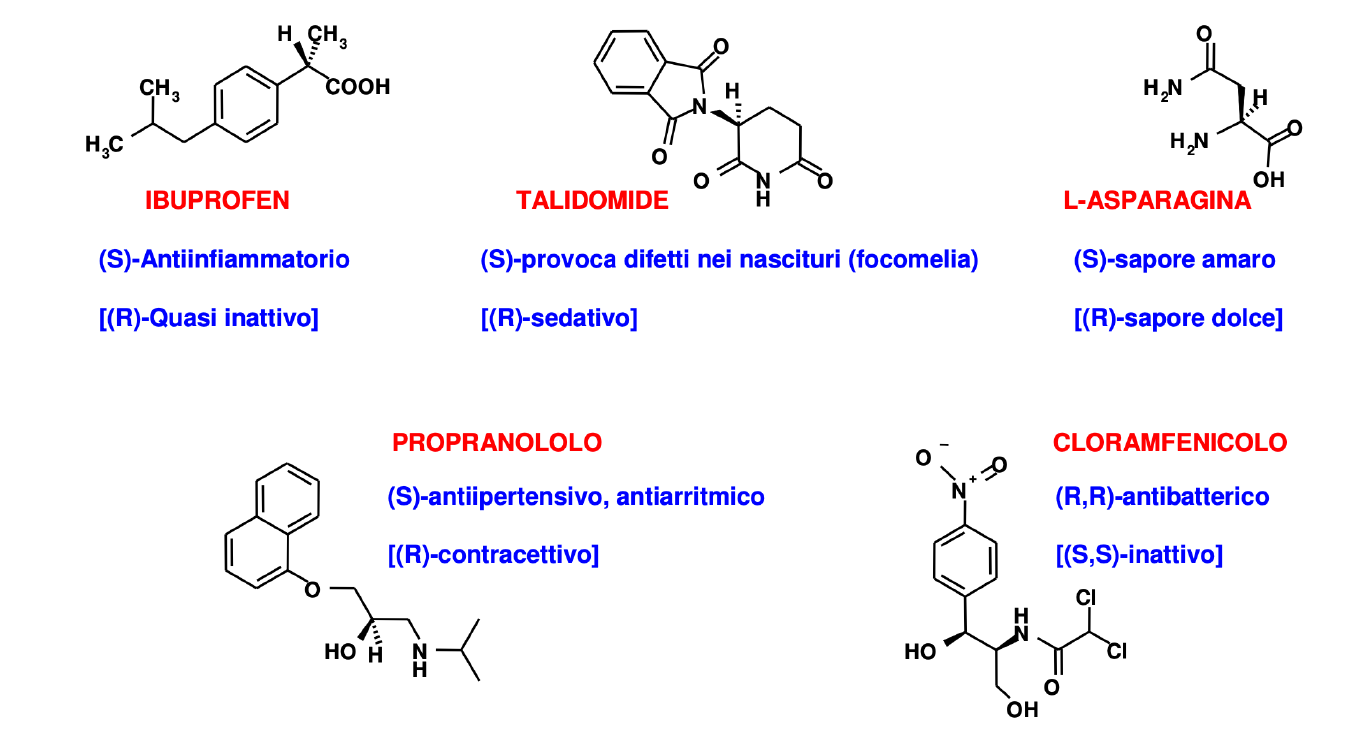
\includegraphics[width=\textwidth]{4_017}
\end{figure}

Se si guardano effetti induttivi, il protone più deschermato è quello
più vicino al carbonile, ovvero il protone in \alpha.
In realtà non è così, in quanto è presente la risonanza. La forma di
risonanza in questione, il protone in a è un protone del doppio legame.
L'altro protone è legato al metile carico positivamente e quindi è
totalmente deschermato.
La forma di risonanza vince sull'effetto induttivo

Questo effetto si vede bene negli aromatici. Prendendo il fenolo, si
vede che per le forme di risonanza hanno le forme in orto e para, i
carboni sono negativi, quindi si ha il massimo dell'effetto schermante e
quindi i protoni non risentono molto dell'effetto del campo magnetico

\paragraph{Ibridazione}

L'elettronegatività aumenta dal carbonio sp\ap{3} a sp, per via del carattere
maggiore del carbonio, in quanto aumenta il carattere s dell'orbitale molecolare.

Dalla serie etano, etene, etino, si vede che l'elettronegatività
aumenta, quando si passa da un carbonio sp\ap{3} ad uno sp\ap{2} ad uno sp.

\paragraph{Anisotropia magnetica}
Come visto precedentemente, l'elettronegatività aumenta passando da un carbonio sp\ap{3} ad uno sp, Però lo spostamento chimico non aumenta proporzionalmente.
Passando da un carbonio sp\ap{3}, si vede un aumento dell'effetto deschermante, però da un carbonio sp\ap{2} ad uno sp si vede che aumenta invece l'effetto schermante. Questo avviene a causa dell'anisotropia magnetica.

Quando si mette il nucleo all'interno di un campo magnetico esterno, si
forza il movimento degli elettroni, creando quindi una corrente diamagnetica.

\fullpicture{4_018}{Anisotropia magnetica nel caso degli alcheni e degli aromatici}{fig:AnMagnAlcheni}

Come si vede in figura \ref{fig:AnMagnAlcheni}, il movimento degli elettroni p è simile per un doppio legame isolato e
per quelli che si trovano nel benzene. La corrente diamagnetica si
oppone al campo magnetico esterno e si somma a quella del campo
magnetico del legame. Diminuisce l'intensità del campo nel legame, ma
aumenta a lato. Quindi il nucleo che è adiacente al doppio
legame è più deschermato, in quanto risente di un campo maggiore.

\halfpicture{4_019}{Anisotropia magnetica nel caso degli alchini}{fig:fig:AnMagnAlchini}

Dalla figura \ref{fig:fig:AnMagnAlchini}, il triplo legame si dispone in modo parallelo al campo magnetico. Il protone del triplo legame è nella zona dove si diminuisce il campo
magnetico esterno, quindi i protoni risultano più schermati e ritornano
alla zona dei protoni alifatici.
Il campo magnetico indotto comporta la diminuzione del campo magnetico
effettivo.

\marginpicture*{4_020}{Cono di anisotropia}

Il cono di anisotropia semplifica il disegno visto prima. La parte che è
fuori dal cono sente di più il campo magnetico e la parte interna del
cono sente un campo magnetico effettivo minore e quindi è più schermata.

Quando si ha un doppio legame si ha la stessa interazione che si avrebbe
con una molecola di benzene.

\fullpicture*{4_021}{Coni di anisotropia per doppi legami \ce{C=C} e \ce{C=O}}

Il protoni dei doppi legami e i protoni degli aromatici, sono più
deschermati del solito. Infatti si trovano rispettivamente da 6 ppm in
poi e da 7 ppm in poi.
Anche i protoni aldeidici sono molto deschermati, per lo stesso motivo
degli alcheni.

\paragraph{Idrogeni acidi}
Si ha un ultimo effetto da vedere, che è l'interazione dei protoni con
l'intorno. Questo si vede anche all'IR, dove si spostavano le bande
dell'alcol e del carbonile.

La presenza del legame ad idrogeno va a spostare il chemical shift. Questo è
causato agli idrogeni acidi, che possono essere coinvolti nel legame ad idrogeno.

Quando un protone forma un legame ad idrogeno, l'idrogeno si allontana
dall'ossigeno, e quindi è più deschermato; si sposta a ppm maggiori.

\halfpicture*{4_022}{Legame ad idrogeno}

Questo effetto dipende da tanti fattori. C'è anche la dipendenza dalla
presenza di acqua, in quanto l'alcol o l'ammina potrà reagire con
l'acqua, spostando il segnale.

Un acido carbossilico si trova a 10-14 ppm. Mentre un ammina/alcol può
variare da 0 a 5 ppm, a seconda di come viene registrato lo spettro.

\begin{figure}[H]
  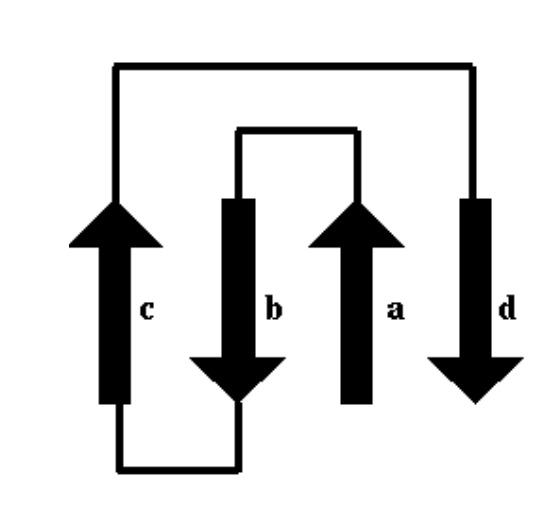
\includegraphics[width=\textwidth]{4_023}
  \caption{Esempi dello spostamento dovuto al legame ad idrogeno.}
\end{figure}

Per l'etanolo, il picco a sinistra è l'idrogeno dell'alcol. Nello spettro dell'etanolo in \ce{CCl4}Si vede che l'alcol è meno concentrato e quindi forma meno legami ad idrogeno, quindi il segnale è più vicino
a zero.

\fullpicture*{4_024}{Spostamento chimico dovuto all'influenza del solvente.}

Se invece il legame ad idrogeno è intramolecolare, la concentrazione non dovrebbe
contare, in quanto il legame si forma all'interno della molecola,
quindi lo spostamento chimico non varia. Questo è un trucco per capire
se c'è idrogeno acido che dà legami intermolecolari

\paragraph{Solvente}

Un'altra cosa importante è il solvente, in quanto le molecole
interagiscono con il solvente. C'è sempre un interazione con il
solvente. La stessa specie con solventi diversi da spettri diversi,
quindi in letteratura va guardato anche il solvente.

\fullpicture*{4_023}{Il chemical shift può variare anche a causa delle interazoni con il solvente}

I segnali non cambiano, però lo spostamento chimico può variare.

\subsection{Riassunto dei chemical shift}

\fullpicture*{2_025}{Schema dei chemical shift per i vari gruppi}

Aggiungendo sostituendi, si aggiungono anche gli effetti induttivi; i gruppi elettronegativi deschermano i protoni che si troveranno sopra due ppm.
Per atomi più elettronegativi, deschermano ancora di più i protoni e si trovano a quattro ppm.
Tra due e tre ppm si trovano gli idrogeni di un alchino terminale.

Sopra i cinque ppm, si trovano i protoni del doppio legame e sopra sette ppm si trovano i protoni aromatici
Dopo si trovano gli idrogeni aldeidici

Gli idrogeni di acidi carbossilici si trovano in ultima posizione, in quanto sono molto acidi e si trovano quasi sempre in dimeri.

I protoni legati tra gli eteroatomi possono spostarsi di tanto, quindi
dipende dall'effetto dei sostituenti.

Gli spostamenti chimici servono per trovare le tabelle degli spostamenti
chimici. Da queste tabelle sono stati dedotti gli spostamenti chimici
per una data molecola, in modo empirico. Si sommano i diversi effetti
dei sostituenti, ovvero l'effetto è cumulativo.

\subsection{Stima dei chemical shift}
Si può  stimare lo spostamento chimico di un protone.

Ad esempio, per i protoni metilenici, c'è la regola si Shoolery. Gli effetti sono tabulati e per ottenere il chemical shift del protone vanno sommati.

Si può usare anche la \emph{regola di Shoolery} per calcolare il chemical shift del metilene. Si nota che se si sostituisce un gruppo con un sostituente, si ottiene un gruppo metile.
\[
  \delta = 0.23 + \sigma(\text{Y}) + \sigma(\text{Z})
\]

Per i protoni olefinici, si ha una formula simile.
\[
  \delta = 5.28 + \sum S(\delta)
\]
Per i protoni aromatici, si ha una formula simile a quella dei protoni olefinici
\[
  \delta = 7.27 + \sum S(\delta)
\]
In questo caso, il chemical shift di base è 7.27, mentre per i protoni olefinici, il valore base è di 5.28

\halfpicture{4_026}{Stima di chemical shift}{fig:Stima}

Applicando queste formule, come si vede nell'immagine \ref{fig:Stima}, è facile stimare lo spostamento chimico. Il valore tra parentesi è il valore sperimentale

Oggigiorno ci sono dei software per calcolare lo spettro NMR di una
molecola.

\section{Integrazione}

L'area viene misurata dallo strumento, e mi da una curva, detta integrale, che misura l'area. Il valore dell'integrale non è assoluto, ma relativa. Lo strumento non sa
distinguere i numeri, solo noi sappiamo integrare nel modo giusto.

\fullpicture{4_027}{Spettro dell'etanolo.}{fig:NEtanolo}

Dallo spettro in figura \ref{fig:NEtanolo}, si vede che il si hanno tre segnali:
\begin{itemize}
  \item Il segnale dai protoni metilici \ce{CH3}
  \item Il segnale dai protoni metilenici \ce{CH2}
  \item Il segnale del protone \ce{O-H}
\end{itemize}
Ci si aspetta di vedere l'area dei segnali in ordine 9:2:1.

Il segnale del protone ossidrilico si vede a 5 ppm, però si può muovere, mentre il segnale del
metile è molto schermato, quindi vicino a 0.
Il segnale dei protoni metilenici sarà anch'esso molto schermato, però meno schermato rispetto ai protoni metilici, in quanto i protoni sono vicini ad un atomo elettronegativo.

\marginbox*{
  Nello spettro \ref{fig:NEtanolo} si vede che il segnale del TMS è posto a zero.
}

Nello spettro dell'etanolo si vedono tre segnali colorati, uno rosso, uno verde e uno blu.
La curva in nero è l'integrale.
Per assegnare le aree si parte dal segnale più piccolo, a cui viene assegnato valore 1. Quindi si vede che l'integrale degli altri segnali vale rispettivamente 2 e 9.
Si possono quindi assegnare i segnali ai protoni.

Nell'esempio in figura \ref{fig:NIncognito}, si parte da dalla formula molecolare, però la struttura non è nota.

\fullpicture{4_028}{Spettro di un composto incognito.}{fig:NIncognito}

I due segnali in rosso e in blu sono degli idrogeni del composto. Misurando le aree, il segnale blu ha un integrale pari a 1, mentre il segnale in rosso ha l'integrale pari a 1.5. Questo è impossibile, in quanto non si può avere un numero non intero di atomi di idrogeno. Per arrivare al numero reale
di protoni, si deve moltiplicare per 4, ottenendo quindi un segnale con sei protoni e uno con quattro  protoni.

Entrambi i due segnali sono molto deschermati, questo potrebbe essere a causa dell'atomo di ossigeno.

\marginbox*{
  Quando si vedono pochi segnali, si vede che la molecola è simmetrica, perché avrà lo stesso intorno chimico.
}

In questa molecola si vede che un segnale è un multiplo di 3; questo consente di assegnare il segnale agli idrogeni di un metile. Inoltre in questo spettro si vede che c'è un secondo segnale che è un multiplo di 2. Quindi si può assegnare questo segnale a dei protoni metilenici.

\marginbox*{
  Se si vedono dei segnali che sono multipli di 3, allora questi saranno i segnali dovuti al metile (o ai metili). Se invece si vede un segnale che è multiplo di 2, allora è possibile che siano i protoni del gruppo metilenico.
}

In questa molecola si vede anche che il grado di insaturazione è pari a zero, quindi si può escludere la presenza di doppi legami o di cicli.

Si può quindi escludere la presenza di chetoni, aldeidi o di alcoli, in quanto i segnali non rientrano nel range di frequenza per questi gruppi. Da qui si può dedurre che la molecola è un etere; per determinare la struttura si deve tenere conto che sono presenti due gruppi \ce{CH3}, due gruppi \ce{CH2}, due atomi di ossigeno eterei. La struttura è
\begin{center}
  \ce{CH3-O-CH2-CH2-O-CH3}
\end{center}

Sia il segnale del metile che quello del metilene sono molto deschermati; questo consente di escludere la formule molecolare
\begin{center}
  \ce{CH3-CH2-O-O-CH2-CH3}
\end{center}
in quanto, in questa formula, i protoni del metilene sono molto più deschermati di quelli del metile.

La molteplicità è diversa per i due segnali. È una conseguenza dello scambio chimico, per via della presenza di tracce di acqua.

\marginbox*{
  I solventi deuterati, se non c'è scritto anidro, sono umidi (tendono ad accumulare acqua). I solventi anidri si prendono sempre sotto flusso di azoto.
}

\section{Accoppiamento scalare di spin}

La struttura fine dei segnali NMR si chiama molteplicità dei segnali; questa struttura ha origine dagli  accoppiamenti di spin.

Quando si sta osservando il nucleo, il nucleo può avere vicino un altro protone, che può essere sia nello stato di spin \alpha{} sia nello stato di spin \beta{}. Se è nello stato \alpha{}, i campi si sommano. Se \beta{}, il campo risentito dal protone è minore, quindi la causa della molteplicità è l'influenza dello stato di spin di un nucleo vicino, del nucleo che si sta osservando.

La molteplicità dà molta informazione, a volte troppa. Se la molteplicità è molto elevata, diventa difficile determinare i segnali, però si può rimuovere con determinati esperimenti.

L'accoppiamento dei nuclei avviene se questi non sono nuclei equivalenti.

\subsection{Sistema di spin $\text{H}_{\text{A}} - \text{H}_{\text{X}}$}

Considerando un sistema di spin formato da due protoni \ce{H_{A}} e \ce{H_{X}}, si vede che il sistema è un insieme di protoni non equivalenti che accpppiano tra loro. Il protone \ce{H_{A}} può trovarsi negli stati di spin \alpha{} e \beta{} con probabilità quasi uguale. Poiché ogni nucleo ha un momento magnetico, il campo magnetico del nucleo \ce{H_{A}} può influenzare quello subito dal nucleo \ce{H_{X}} e questa influenza è opposta se il nucleo \ce{H_{A}} è nello stato \alpha{} o \beta{}.

Questo sistema di spin è più semplice, in quanto è il sistema con meno protoni diversi.

\begin{figure}[H]
  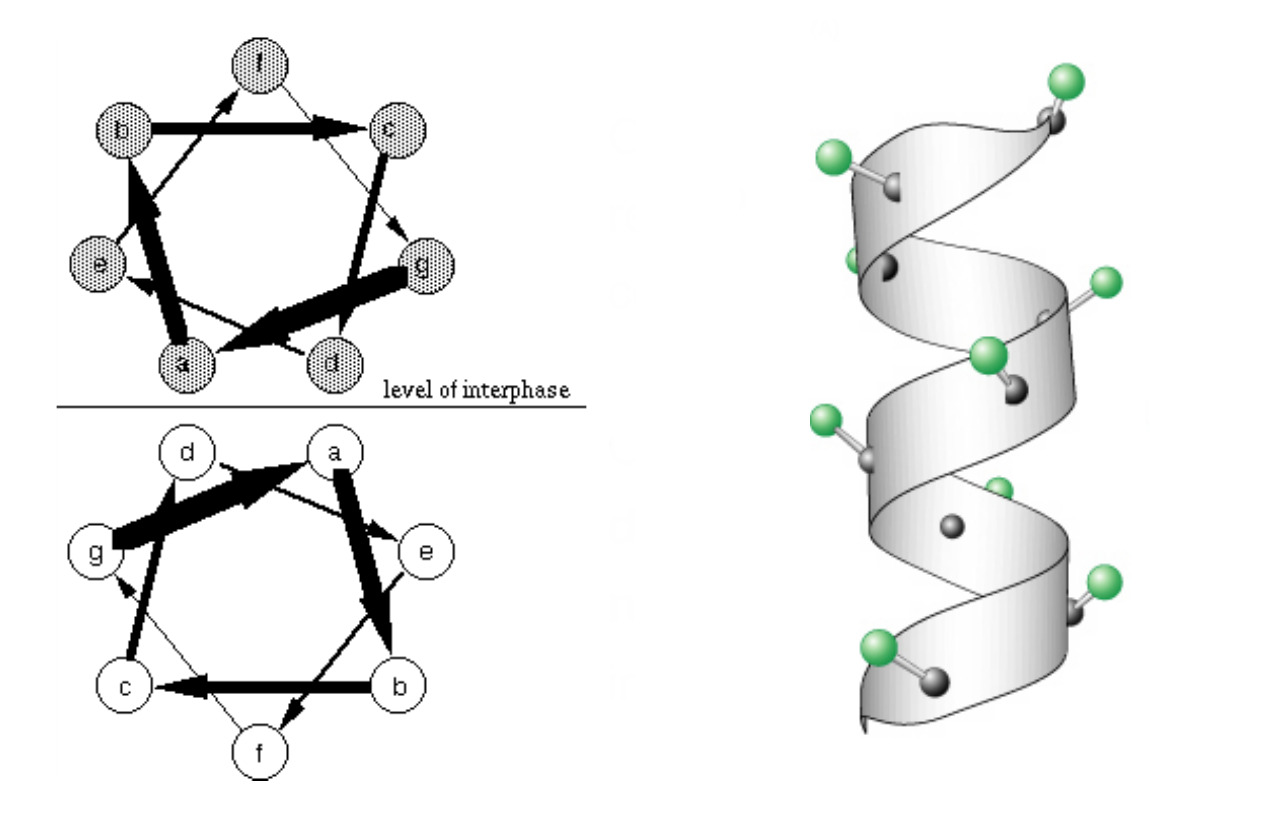
\includegraphics[width=0.5\textwidth]{4_029}
\end{figure}

\ce{H_{X}} risuona quindi a frequenze un po' diverse se si trova vicino ad un idrogeno \ce{H_{A}} nello stato \alpha{} o nello stato \beta{}.
Il protone \ce{H_{X}} dà origine a due segnali, che nel loro complesso vengono detti \emph{doppietto}. Il numero di linee in cui è diviso il segnale generato da un nucleo è detto quindi \emph{molteplicità del segnale}

\marginbox*{
  Per avere un sistema \ce{H_{A}-H{X}} è necessario che i protoni abbiano un chemical shift molto diverso tra loro. La differenza di frequenza deve essere maggiore di \[ \frac{\Delta \nu}{\text{J}} = 10 \text{Hz} \]
}

Tutti i discorsi fatti possono essere ripetuti all'inverso considerando l'influenza di \ce{H_{X}} sulla frequenza di risonanza di \ce{H_{A}}, e allo stesso modo si può concludere che anche il segnale di \ce{H_{A}} è un doppietto. Il doppietto è un segnale che presenta due rami con la stessa intensità. 

La distanza (differenza di frequenza, Hz) tra i due segnali del doppietto (di solito detti rami del doppietto) è detta costante di accoppiamento ed indicata col simbolo $J$. Anche la costante $J$ dà informazioni strutturali. 
La frequenza di risonanza del nucleo si trova a metà dei due picchi del doppietto.

Per calcolare la costante di accoppiamento si può
partire dai ppm del segnale. Si misura la distanza in ppm tra le due righe in ppm e poi si moltiplica la differenza per la frequenza di lavoro dello strumento.

L'accoppiamento è sempre reciproco. Se \ce{H_{A}} è accoppiato con \ce{H_{X}}, anche \ce{H_{X}} è accoppiato con \ce{H_{A}}. Si dice che \ce{H_{A}} e \ce{H_{X}} sono accoppiati tra loro.

La costante di accoppiamento tra \ce{H_{A}} e \ce{H_{X}} è identica a quella tra \ce{H_{X}} e \ce{H_{A}}.L'accoppiamento è indipendente da \(B_0\). La costante di accoppiamento viene misurata in Hz, non in ppm.

\marginbox*{
  L'accoppiamento degli spin avviene sempre, però se lo spettro è stato preso con uno strumento a bassa risoluzione, non sempre si riesce a distinguere la struttura fine degli spettro.
}

Questo accoppiamento di spin si chiama accoppiamento scalare. Perché è
un'interazione che appare attraverso i legami, non attraverso lo spazio.

\marginbox*{
  Le costanti di accoppiamento sono indipendenti dal campo magnetico; la scala dei ppm però ne è dipendente.
  Quindi, più uno spettro è ad alta risoluzione, più la struttura di un segnale è vicina.\\
  Il risultato è che le costanti di accoppiamento sembrano diminuire quando il campo magnetico esterno aumenta.
}

Se il numero di legami aumenta, l'effetto dell'accoppiamento scalare diminuisce. Per il protone, si vede l'accoppiamento tra protoni non-equivalenti separati da due legami (protoni legati allo stesso carbonio, detti anche protoni geminali, con costante \ap{2}J). Questo accoppiamento si vede solo in determinati
casi, ovvero se i due protoni sono diastereotopici.

Si può anche vedere un'accoppiamento tra protoni separati da tre legami, che quindi vengono chiamati protoni vicinali, con costante di accoppiamento \ap{3}J.
In altre strutture si possono vedere anche accoppiamenti \ap{4}J e anche \ap{5}J.

\begin{figure}[H]
  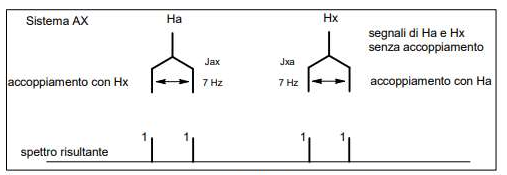
\includegraphics[width=\textwidth]{4_030}
  \caption{Albero di frazionamento}
\end{figure}

Il modo più semplice per capire l'accoppiamento è usare l'albero di frazionamento. In questo albero i segnali originali stanno sopra, e via via che si accoppiano gli spin si aumentano i rami.

\paragraph{Sistema di spin $\text{H}_{\text{A}} - \text{H}_{\text{X}_2}$}

Prendendo come esempio un secondo sistema, ovvero \ce{H_{A}-H_{X2}} si vede che l'albero di frazionamento cambia, in quanto un protone accoppia con due protoni equivalenti.

Nell'albero di frazionamento si vede che i protoni \ce{H_{X}} formano un doppietto, in quanto accoppiano con un solo protone

\begin{figure}[H]
  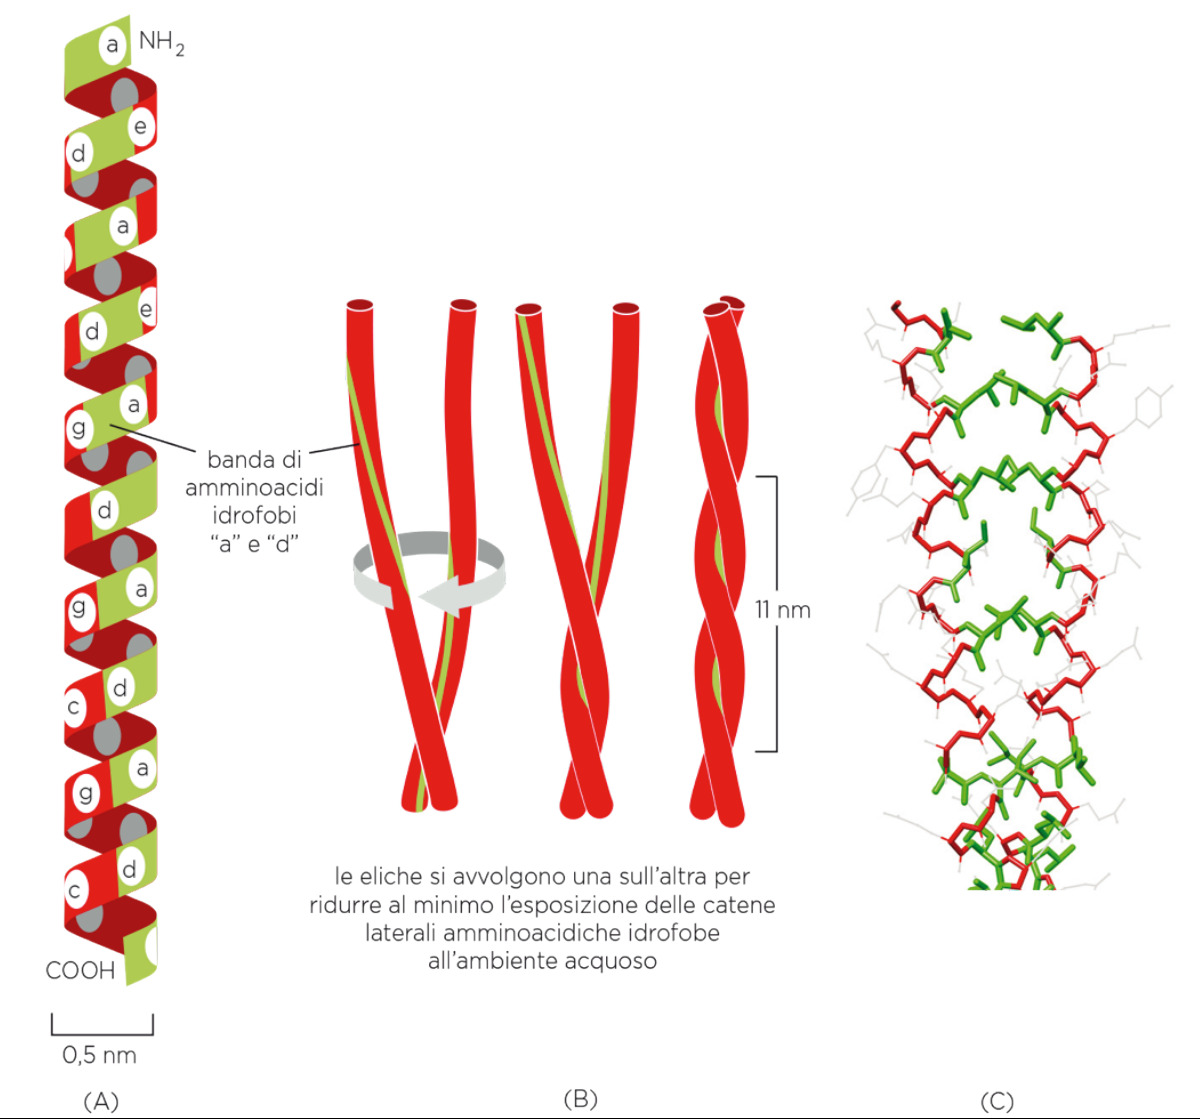
\includegraphics[width=\textwidth]{4_031}
\end{figure}

I protoni \ce{H_{A}} invece formano un tripletto (con molteplicità 3). Il sistema è \ce{AX2}.

I sistemi più complicati si possono analizzare allo stesso modo. Ad esempio, nel sistema \ce{A2X3} si vede che il segnale di A è un quartetto, e il
segnale di X è un tripletto.
La molteplicità, ovvero il numero di segnali fini, è uguale a \(2NI+1\), dove $N$ è il numero dei nuclei più vicini, mentre $I$ è il il numero quantico di spin del nucleo.
\begin{figure}[H]
  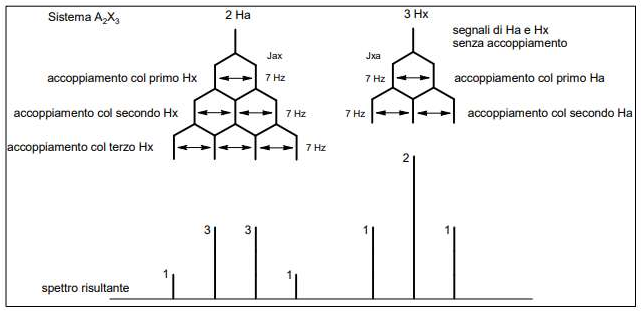
\includegraphics[width=\textwidth]{4_032}
\end{figure}

Per sapere l'intensità dei segnali relativa si usa il triangolo di Tartaglia.

\subsection{Sistemi con tre protoni non-equivalenti}

Lo spostamento chimico deve essere diverso, per i tre protoni. Il sistema si chiama \ce{AMX}. Non vale più la regola \(2NI+1\). Bisogna considerare i diversi accoppiamenti, in serie. Si avranno quindi multipletti (AM) di multipletti (AX).

\begin{figure}[H]
  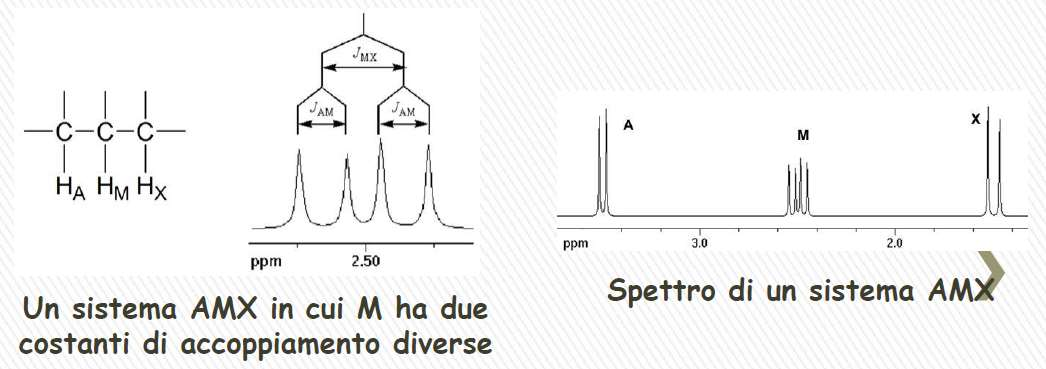
\includegraphics[width=\textwidth]{4_033}
\end{figure}

Per capire da dove iniziare, si va a guardare la costante di accoppiamento. Per analizzare questo tipo di sistemi, è importante ricordare i diagrammi di frazionamento.

Per un semplice sistema AMX, si può pensare a una catena lineare. A e X non accoppiano, però M accoppia con tutti e due. Per risolvere questi sistemi è necessario stabilire un ordine nelle costanti di accoppiamento. In questo caso
\[
  \text{J}_{\text{AM}} < \text{J}_{\text{XM}}
\]

Si vede quindi che il protone M accoppia con il protone X per dare un doppietto, e poi accoppia con A per dare un altro doppietto. Idealmente, si dovrebbe trovare un doppietto di doppietti. Le intensità sono 1:1:1:1.

Bisogna sempre iniziare dalla costante di accoppiamento più grande, per poi fare gli accoppiamenti con constanti via via calanti.

\begin{figure}[H]
  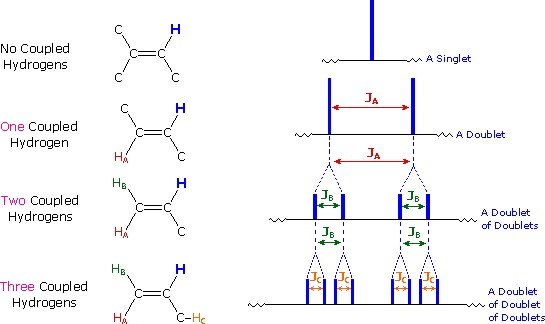
\includegraphics[width=\textwidth]{4_034}
\end{figure}


Nella figura, si vede che l'accoppiamento nella prima e nella seconda molecola sono banali.
Nel terzo caso, si vede che è presente un doppietto di doppietti. Si può anche aggiungere un quarto idrogeno; in questo caso, si avrà un doppietto di doppietti di doppietti, partendo dalla costante più grande fino a quella più piccola.

\marginbox*{
  I multipletti del primo ordine sono quasi sempre centro-simmetrici ed la costante di accoppiamento più piccola è la prima che si può misurare, in quanto basta fare la differenza dei picchi consecutivi.
}

Si possono analizzare anche sistemi più complicati, come per un chetone \alpha,\beta-insaturo.
Quindi si vede che i protoni del metile sono equivalenti, mentre quelli del gruppo metilenico non lo sono. Il sistema è \ce{AMX3}

\begin{figure}[H]
  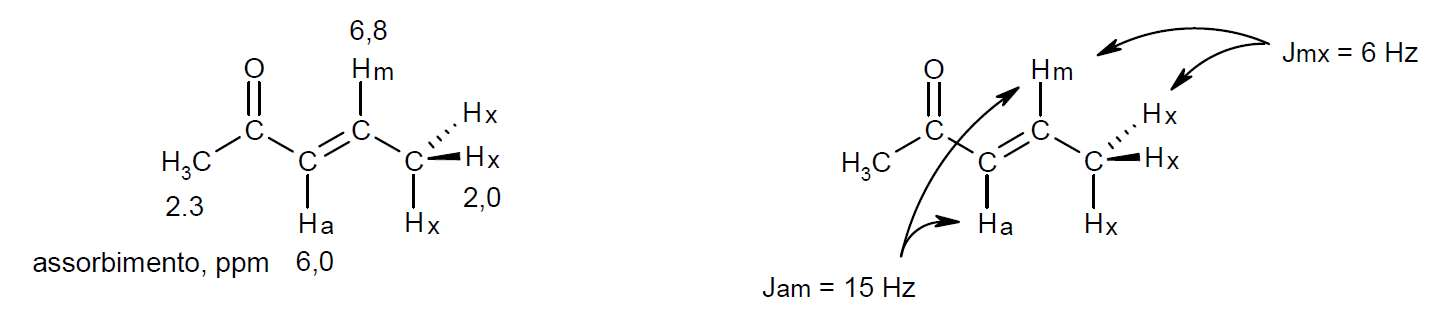
\includegraphics[width=\textwidth]{4_035}
\end{figure}

I protoni A e X accoppiano solo con il protone M, mentre il protone M accoppia sia con A che con X. Il segnale M sarà un doppietto di quartetti. L'ordine dei multipletti dipende dalla costante di accoppiamento; se le costanti sono inversite, allora il segnale per il protone M diventerà un quartetto di doppietti.

\marginbox*{
  Nel caso dei multipletti sovrapposti, è difficile trovare l'area e la corrispondente molteplicità. Si ricordi che le costanti J non cambiano, quindi bisogna guardare la distanza dei segnali.
}

\fullpicture{4_036}{Spettro NMR al protone di un aldeide alifatica}{fig:AldAlifNMR}

Nello spettro dell'aldeide alifatica in figura \ref{fig:AldAlifNMR}, ci sono tre tipi di protoni, quindi ci si aspettano tre segnali.

L'idrogeno aldeidico, accoppia con il protone della ramificazione, mentre i protoni dei gruppi metilici accoppiano con il protone della ramificazione. Il protone della ramificazione accoppia con tutti e due.

Se il protone della ramificazione accoppia prima con i gruppi metilici, si avrebbe un settetto di doppietti, mentre se accoppia prima con il protone aldeidico, si avrebbe un doppietto di settetti. Nello spettro, si vede che si ha un settetto di doppietti.

\subsection{Informazioni strutturali}
Si può anche vedere l'informazione strutturale, che deriva dalla costante di accoppiamento.

Le costanti di accoppiamento che si possono vedere per il protone sono quelle vicinali e germinali. Raramente si possono vedere accoppiamenti a cinque/sei legami.

La costante di accoppiamento può essere negativa o positiva, però non importa, in quanto si prende sempre il valore assoluto.

\url{
  https://www.chem.wisc.edu/areas/reich/chem605/index.html
}
Si possono vedere i valori delle costanti di accoppiamento, in questo sito.

\begin{figure}
  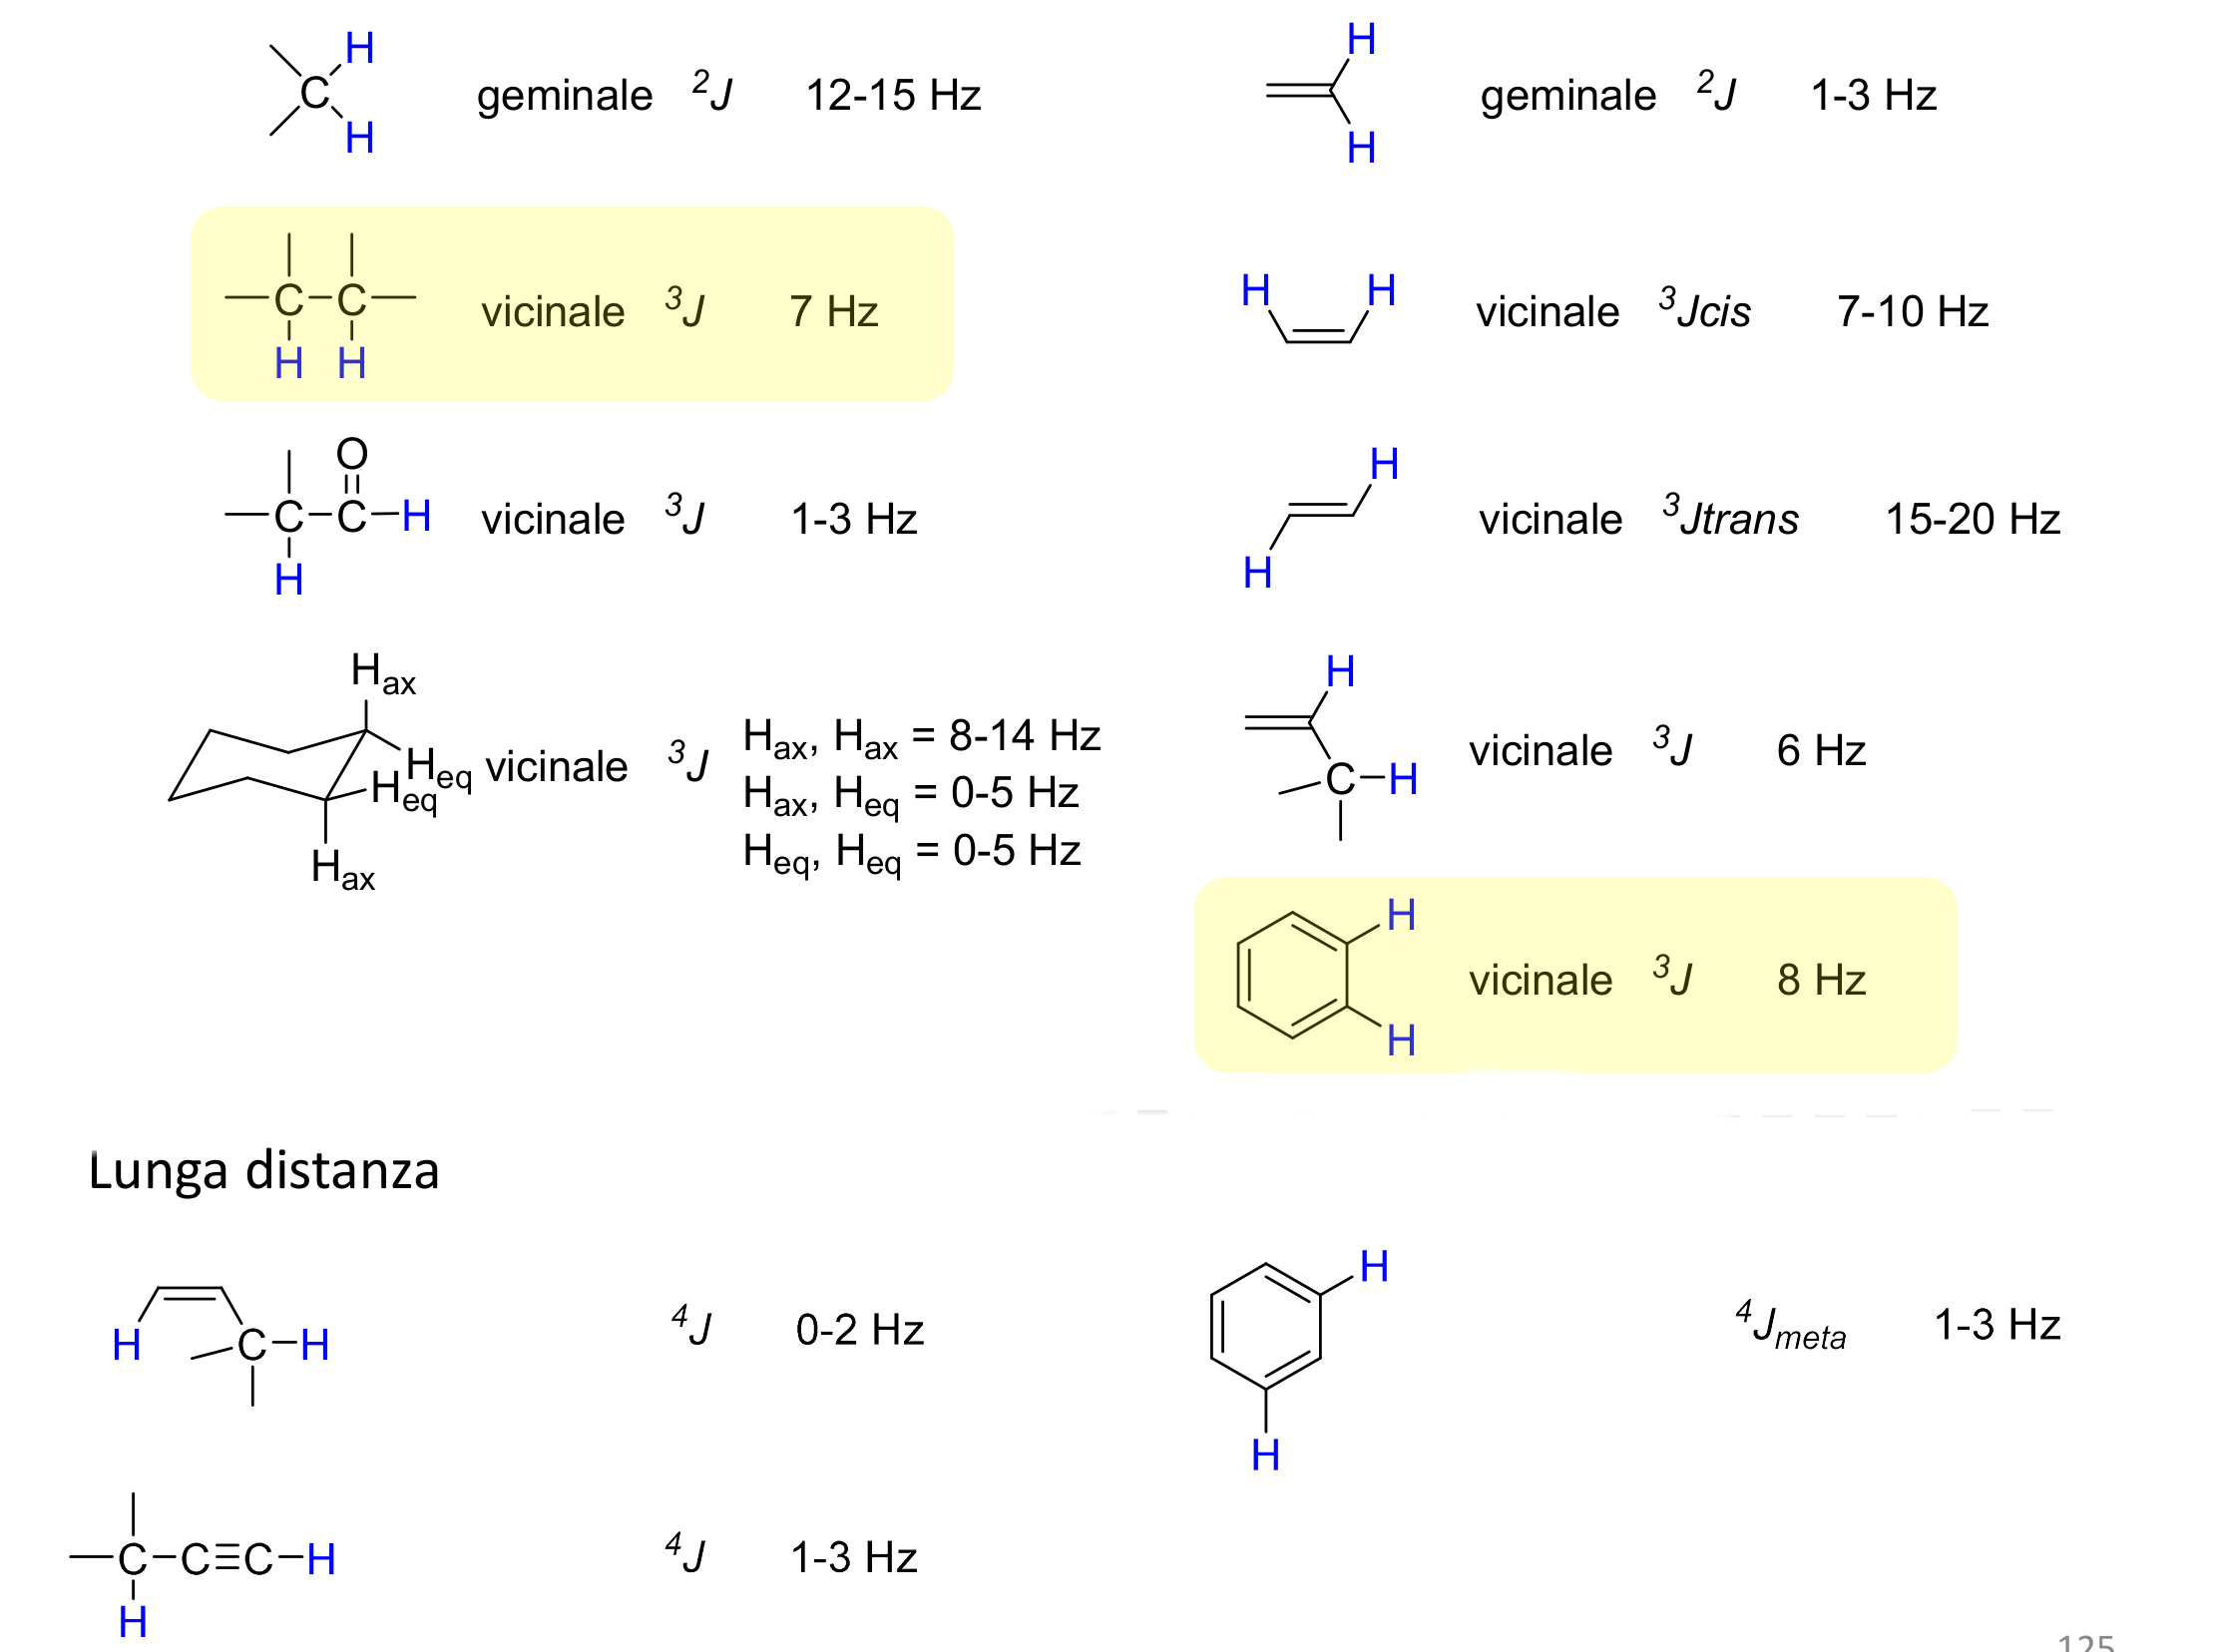
\includegraphics[width=\textwidth]{4_037}
\end{figure}

Per le costanti di accoppiamento geminale legato ad un carbonio sp\ap{3}, si hanno costanti nell'ordine di 12-15 Hz, che sono considerate molto alte. Per il protone geminale legato a un carbonio sp\ap{2}, si parla di 1-3 Hz.

Le constanti di accoppiamento vicinale per un carbonio sp\ap{3} sono di circa 7 Hz. Per un carbonio sp\ap{2}, la costente vicinale dipende dall'intorno chimico. Se si è in presenza di un accoppiamento aldeidico, le costanti sono dell'ordine di 1-3 Hz.

Nel doppio legame, la costante dipende dalla conformazione relativa. Per la conformazione cis si hanno 7-10 Hz, mentre per la conformazione trans, si hanno costanti molto elevate (15-20 Hz). Le costanti tra un protone alifatico e uno olefinico è di circa 6 Hz.

Quando si ha un ciclo o una conformazione rigida la costante tra i due protoni vicinali è diversa in base alla posizione (assiale o equatoriali). Tra protoni assiali si ha una grande costante di accoppiamento, mentre più è coinvolto il protone equatoriale e più la costante si abbassa.

Due protoni aromatici vicinali hanno un valore di costante di accoppiamento a metà tra quello di un singolo e di un doppio legame, ovvero circa 8 Hz.

\marginbox*{Le costanti di accoppiamento di due protoni aromatici consentono di determinare la disposizione dei protoni nel ciclo.}

In un sistema aromatico è possibile vedere anche gli accoppiamenti a lunga distanza (ovvero a quattro/cinque legami. In tali sistemi è possibile vedere una costante \ap{4}J, che corriponde ad una disposizione in meta dei protoni. Inoltre, in questi sistemi è possibile vedere anche un accoppiamento \ap{5}J, che corrisponde ad una disposizione in para dei protoni

Questi accoppiamenti sono anche visibili in presena di sistemi rigidi, ovvero di doppi o tripli legami.
Si riesce a vedere un protone con una costante \ap{4}J in un alchene, però la costante è molto bassa.

Il valore della costante di accoppiamento J cambia perché sono presenti diversi effetti:
\begin{itemize}
  \item Il primo effetto riguarda il valore dell'angolo diiedro tra i protoni che danno accoppiamento.
  \item Il secondo effetto dipende dalla presenza di gruppi elettron-donatori o elettron-accettori.
\end{itemize}

Per un gruppo elettron-donatore, la costante aumenta, mentre se è presente un gruppo elettron-accettore, la costante diminuisce.
Questo si vede in modo particolare nei protoni aldeidici, dove la presenza dell'ossigeno fa abbassare la costante di accoppiamento.

La costante di un sistema alifatico dipende dalla disposizione dell'angolo diedro. L'interazione si misura nell'equazione di Karplus.
\[
  \text{J}_{HH'} (\phi) = A + B \cos \phi + C \cos 2\phi
\]

\halfpicture{4_038}{Grafico dell'equazione di Karplus}{fig:Karlplus}

Il grafico \ref{fig:Karlplus}, dice che quando l'angolo è di 90° la costante è molto piccola. Se invece l'angolo è 180 o 0 °, la costante è molto grande.

\fullpicture{4_039}{Equazione di Karplus nel cicloesano}{fig:KarlplusCiclo}

Ad esempio nel grafico \ref{fig:KarlplusCiclo}, gli accoppiamenti tra protoni assiali sono molto più grandi degli accoppiamenti tra protoni equatoriali.
Si vede che le interazioni tra protoni assiali (180°) è massima, mentre per i protoni equatoriali, l'interazione è bassa. 

Questa equazione può essere usata per fare degli studi sulla struttura.

Questo avviene a causa della sovrapposizione degli orbitali. L'effetto dello spin si propaga attraverso i legami. Nell'angolo diiedro può esserci una sovrapposizione maggiore o minore degli orbitali. Più grande è la sovrapposizione, più facile è la propagazione dell'effetto dello spin.

Quando l'angolo è a 90° o 60°, non c'è una buona sovrapposizione, in quanto gli orbitali non sono paralleli.

Quest'equazione spiega anche la differenza tra le costanti di accoppiamento in un alchene cis e in un alchene trans; entrambi gli accoppiamenti dovrebbero essere intensi.

Tuttavia, si vede che nel composto cis gli orbitali si stanno separando, mentre nel composto trans, gli orbitali sono paralleli, il che consente agli orbitali di sovrapporsi meglio.

\begin{figure}
  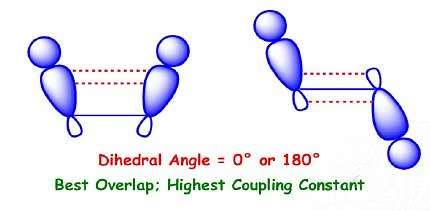
\includegraphics[width=0.5\textwidth]{4_040}
\end{figure}

\subsection{Accoppiamenti a lunga distanza}

Si osserva in sistemi insaturi, o aromatici. La \ap{5}J si può vedere in soli sistemi aromatici. La costante di accoppiamento è piccola, quindi lo strumento deve avere la risoluzione necessaria per distinguere i segnali.

\marginpicture*{4_041}{In questa molecola si vedono quattro segnali}

Si ha un'interazione \ap{4}J. Ci si aspettano quattro segnali. Partendo da destra i sinistra, si numerano i protoni (a,b,c,d).

Per i protoni a, si vede che i protoni sono molto deschermati; la molteplicità è pari a 1.

Per il protone b, darà un segnale sopra i 5 ppm. È un doppietto di quartetti. La prima costante è elevata (con l'altro protone c), mentre con quelli del metile, ci sarà una costante più bassa.

Per il protone c, si può vedere un doppietto di quartetti, in quanto il portone è in trans. Il protone più deschermato è c, in quanto c'è la risonanza, per cui il segnale di c è a ppm più elevati.

I protoni d, danno un doppietto di doppietti. È a 2-4 ppm, in quanto è legato ad un doppio legame, e quindi può essere un pò deschermato.

Nel segnale più deschermato, si vede che si ha un doppietto di quartetti. Per calcolare J, si va a vedere la differenza prima della J più piccola, e poi la J più elevata.

\begin{figure}
  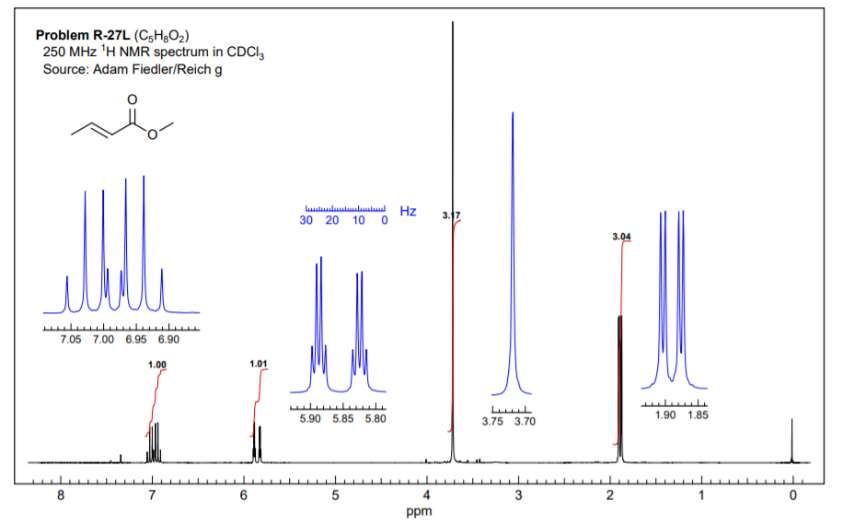
\includegraphics[width=\textwidth]{4_042}
\end{figure}

\paragraph{Accoppiamento con altri nuclei}

C'è accoppiamento eteronucleare se questo nucleo è un nucleo molto abbondante. Se è poco abbondante, non si vede il segnale, in quanto è poco probabile averli nella stessa molecola. Inoltre, $I$ deve essere uguale a 1/2, gli eteronuclei possibili sono \ce{^{14}F} e il \ce{^{31}P}.

Si vede il \ce{^{14}F} in quanto è l'isotopo più abbondante e ha spin 1/2. Si
vede che l'accoppiamento è molto grande 150-200 Hz.

\begin{figure}
  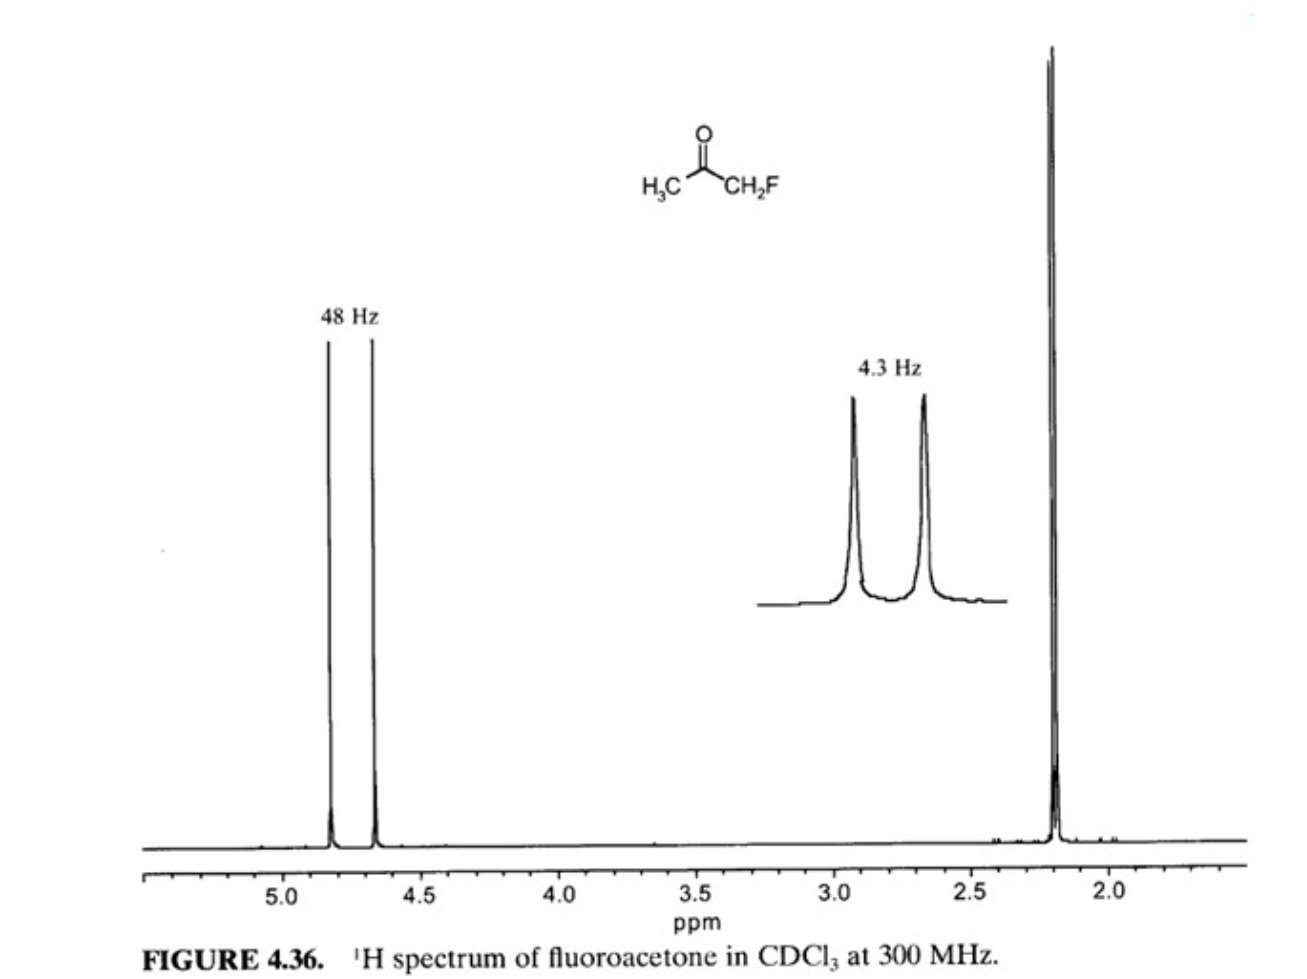
\includegraphics[width=\textwidth]{4_043}
  \caption*{Nello spettro, ci si aspetterebbe due singoletti. In realtà, il fluoro
  consente di vedere due doppietti, separati con una J diversa}
\end{figure}

Con il fosforo, si hanno costanti dell'ordine di 700 Hz.

Con il carbonio 13, non si vede l'accoppiamento, perché è poco
abbondante.

\subsection{Sistemi di secondo ordine}

I sistemi di secondo ordine non sono analizzabili con i metodi usati per i sistemi del primo ordine. Un sistema del secondo ordine è caratterizzato da una differenza di costante di accoppiamento pari a \[ \frac{\Delta \nu}{\text{J}} = 10 \text{Hz} \]

Un sistema di secondo ordine è anche un sistema dove i protoni sono chimicamente equivalenti ma non magneticamente equivalenti.

\marginpicture{4_045}{Si vede la progressione del sistema AX che diventa AB. Quando
diminuisce la differenza di frequenza, si nota che c'è un cambio di
segnale.}{fig:EffTetto}

Un sistema di secondo ordine è indicato con le lettere AB e i suoi protoni sono indicati come \ce{H_{A}} e \ce{H_{B}}. Il sistema passa quindi da AX ad AB in quanto gli accoppiamenti sono molto simili


Nella figura \ref{fig:EffTetto}, si vede quindi che i rami esterni diminuiscono, mentre i rami
interni aumentano di intensità. Questo si chiama effetto tetto.
Man mano che la frequenza diminuisce, l'effetto tetto aumenta, fino ad
arrivare all'estremo.
Il caso limite è quello che non c'è differenza di frequenza, i due
protoni appaiono alla stessa frequenza e non accoppiano.

In un sistema AB, la differenza tra i due rami è la stessa e può essere
calcolata da entrambi i segnali.

Lo spostamento chimico del segnale cambia, non è più uguale al centro
dei multipletti, ma si vede che man mano che la frequenza diminuisce, il
centro si sposta e si avvicina al ramo con più intensità.

Quindi è il ``centro di massa'' del segnale, lo spostamento chimico del
multipletto.

Questo sistema di secondo ordine è tale perché dipende dalla frequenza
del campo magnetico. A seconda della frequenza di funzionamento dello
strumento, si possono avere dei sistemi di primo o di secondo ordine.

La frequenza nelle immagini cambia da 600 a 100 MHz.

Più la frequenza è bassa e più è possibile che si veda un sistema del
secondo ordine.

Quindi se ci si ritrova con uno spettro di secondo ordine, il primis, si
cambia strumento; si usa uno strumento più potente. È possibile che il
sistema diventi del primo ordine.

Se questo non funziona, allora è difficile ottenere i valori di
spostamento chimico. Si usa la formula sotto

\[
  \Delta\nu AB = (\nu A - \nu B ) = \sqrt{(\nu_1 - \nu_4 )(\nu_2 - \nu_3 )} \text{Hz}
\]

Per risolvere il sistema, si guarda sempre la distanza tra i due rami.
Dopo, per riuscire a determinare la posizione esatta del protone in a e
in b, si calcola la differenza con queste equazioni (rami esterni) e poi
si applica la formula vista prima.
\[
  \nu_A = \nu_C + \nicefrac{1}{2} (\Delta\nu_{AB}) \text{Hz}
\]
\[
  \nu_B = \nu_C + \nicefrac{1}{2} (\Delta \nu_{AB}) \text{Hz}
\]

Se ci si trova un sistema AB, come si fa a descrivere questo sistema? La
cosa migliore è fare i calcoli; però questo non si fa quasi mai, in quanto non serve complicarsi la vita.

Si dà il centro dei due segnali, e poi si integra per due protoni. Se si usa questa procedura, si
dice quindi che si ha un quartetto di un sistema AB.

Si può anche guardare il multipletto come se fosse un sistema del primo
ordine (ma si indica sempre che si ha un multipletto di un sistema AB).

I sistemi con secondo ordine possono essere più complicati. Ad esempio,
si passa da AX2 a AB2, il multipletto diventa difficile da analizzare.

\marginbox*{
  Quando non si sa dare il nome, si dice che è il multipletto, e la frequenza si indica come intervallo di frequenze, perché non si riesce a trovare il chemical shift del multipletto.
}

Si può anche fare il procedimento opposto, partendo da un sistema di
secondo a uno del primo aumentando la frequenza operativa dello
strumento.

\fullpicture{4_047}{Per un sistema ABX, solo due chemical shift cambiano e si avvicinano. Il
multipletto ottenuti è complicato.}{fig:ABX}

Nell'immagine \ref{fig:ABX}, il sistema di secondo ordine più comune è quello dato da due protoni di
un metilene, che sono diastereotopici, in quanto c'è un centro chirale
nella molecola.



\subsection{Protoni magneticamente non equivalenti.}

Per sapere se i protoni sono magneticamente equivalenti bisogna guardare
le costanti di accoppiamento.

\marginpicture*{4_048}{Alchene disostituito}

Ad esempio guardando un alchene disostituito, si vede che i protoni A e B sono
chimicamente equivalenti, però visto che un idrgeno è cis, mentre
l'altro è trans, si vede che ci sono due costanti differenti. Quindi
bisogna guardare il chemical shift vero e proprio.
I protoni sono quindi equivalenti per simmetria, però la costante di accoppiamento è
differente.

I due protoni formano un sistema del secondo ordine. Questo si vede
spesso nei sistemi aromatici.

\marginpicture*{4_049}{Sistema para-sostituito}

Ad esempio, un sistema para-sostituito, si è visto che il doppietto era
``sporco'', nel senso che aveva dei segnali aggiuntivi alla base. Questo
però è dovuto ai sistemi di secondo ordine, e in particolare ai protoni
non equivalenti.

In un anello orto para-sostituito, si hanno quattro protoni (due sopra e
due sotto). Si numerano i protoni come H\ped{a} e H\ped{a}' (sopra) e H\ped{b} e H\ped{b}'
(sotto).

Il protone B accoppia con A e A', però hanno due costanti
di accoppiamento diverse, quindi sono chimicamente uguali, ma
magneticamente non equivalenti.

Questo serve per capire che negli aromatici si trovano multipletti molto
complicati.


\section{NMR in regime di scambio}

L'NMR è una tecnica che permette di studiare sistemi dinamici (equilibri
conformazionali, o isomerizzazioni).

Si può studiare questi fenomeni, in quanto la scala dei tempi dell'NMR
permette di vedere i due segnali nel tempo.

Questi sono processi lenti nella scala dell'NMR; lenti dipende anche dal
tipo di isomero e dallo strumento. I processi con millisecondi vanno
bene.

Tipicamente si riescono a studiare processi nell'ordine dei millisecondi
o nanosecondi.

Quando si ha un equilibrio, ci si può spostare con la temperatura;
quindi giocando con la temperatura, si vede che i processi possono
essere rallentati.

Nell'NMR si lavora a temperatura ambiente controllata 25 °C. Si può
andare sopra la temperatura, però dipende anche dal solvente
(diclorometano, bolle a 66 °C). Inoltre dipende anche dallo strumento
(plastica o altro materiale).

Si vede anche che l'NMR è in flusso d'aria; per raffreddare si utilizza
l'aria, che prima passa nell'azoto liquido, si può arrivare a -200 °C.

\fullpicture{4_057}{Spettro dell'alcol etilico in regime di scambio}{fig:EtOHNMR}

Parlando del protone, si può vedere che i protoni acidi possono essere
scambiati. I protoni vengono scambiati con le tracce di acqua presenti.

Prendendo l'etanolo, come in figura \ref{fig:EtOHNMR}, ci si aspetta di vedere tre segnali: si dovrebbe
avere un doppietto di quartetti (se il H del metilene accoppia con tutti
e due i protoni).

Analizzando lo spettro, però non si vede l'accoppiamento con il protone
del \ce{OH}; c'è uno scambio dei protoni dell'acqua con quelli dell'alcol,
quindi si vede un singoletto senza accoppiamento. Il protone entra ed
esce dalla molecola, velocemente.
Quando lo spettro è privo di acqua, si può vedere lo spettro accoppiato
dell'alcol.

Quindi si vede che alcoli e ammine non danno accoppiamenti in generale.
Mentre il protone di un ammide non è acido e quindi riesce ad
accoppiare.

Questo scambio è utile, in quanto si può utilizzare scambio per
eliminare un segnale. Se si utilizza acqua deuterata, questa scambia il
deuterio con il composto e ne elimina il segnale, come si vede nello spettro \ref{fig:NMRScambioAcido}. Nello spettro sparisce il segnale di \ce{OH}, in quanto il D non può essere
visto all'NMR.

\fullpicture{4_058}{Scambio di un protone acido}{fig:NMRScambioAcido}

\marginbox*{
  Questo esperimento serve per assegnare un singoletto; se il singoletto è alcolico o amminico (o anche di un acido carbossilico), allora scambia, mentre, se non è acido no.
}

Un altro processo visto nell'NMR è si analizza ad esempio, la
dimetilformammide. I due metili dovrebbero essere equivalenti, però l'energia per girare
attorno al singolo legame è alta, in quanto il legame ha un parziale
carattere di doppio legame; questo non consente di ruotare il legame.

\begin{figure}[H]
  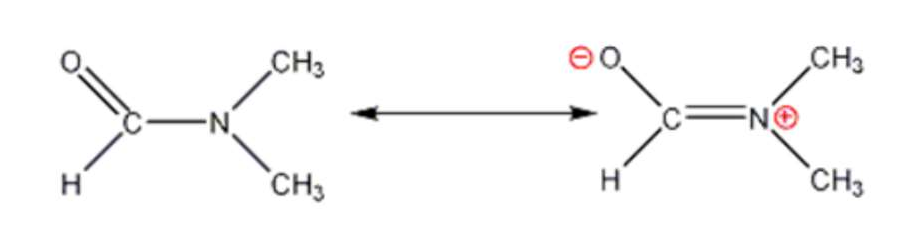
\includegraphics[width=0.5\textwidth]{4_059}
\end{figure}

Questo consente di avere un intorno chimico differente (magneticamente
accoppiato).

Aumentando la temperatura, questo processo diventa veloce (si fornisce
energia al sistema). Quindi si vede che man mano aumenta la temperatura,
i due singoletti si avvicinano, fino alla quale i due segnali si
fondono. Questo fenomeno si chiama coalescenza.

Se si continua a scaldare, allora il sistema diventa un singoletto per
tre protoni, come in figura \ref{fig:NMRCoalescenza}

\fullpicture{4_060}{Fenomeno della coalescenza}{fig:NMRCoalescenza}

Lo spostamento chimico, visto che è un sistema del primo ordine, quindi deve
coincidere tra i due multipletti.
Prima si trova la J più piccola, che è la distanza del primo
multipletto.
La seconda J si trova come distanza tra rami equivalenti. I valori di J
sono differenti, in quanto si hanno due accoppiamenti differenti; un accoppiamento geminale e un accoppiamento a lunga distanza \ap{4}J.

Lo spostamento chimico va calcolato, e va dichiarato nello spettro NMR.
Se si trova la stessa J per dei segnali, allora appartengono allo stesso
multipletto.
Se non si ritrova la stessa distanza, allora si è sbagliato a calcolare
la costante di accoppiamento.

Le assegnazioni vanno fatte con una tabella; va indicata la tipologia di
spettro (\ap{1}H o \ap{13}C, o altro), il solvente e la frequenza di lavoro.

\section{Spettroscopia NMR 13C}

Le differenze più importanti tra \ap{1}H e \ap{13}C sono:
\begin{itemize}
  \item Il segnale è poco intenso, per via della bassa presenza di \ap{13}C.
  \item La costante giromagnetica è molto più piccola rispetto al protone.
  Questo influisce sulla sensibilità della tecnica. Serve più tempo per
  fare uno spettro al \ap{13}C.
  \item La differenza è anche nello spostamento chimico. Normalmente i protoni
  appaiano tra 0 e 14 ppm, quindi a volte i segnali si sovrappongono. Nel   \ap{13}C si ha un range molto allargato 0-200 ppm. Il riferimento è sempre lo
  stesso, e darà il segnale a 0 ppm.
  \item Gli accoppiamenti sono differenti; il protone accoppiare con altri nuclei, se sono
  abbondanti.
\end{itemize}

L'accoppiamento \ap{13}C-\ap{13}C non si vede, perché è poco abbondante, però si
vede l'accoppiamento \ap{13}C-\ap{1}H. Si vedono bene gli accoppiamenti \ap{1}J, ovvero
i sistemi dove \ap{1}H è legato direttamente a \ap{13}C. L'accoppiamento è del
primo ordine.

Questa informazione è molto importante, in quanto si possono differenziare \ce{CH3} da \ce{CH2} da \ce{CH} da \ce{C} come in figura \ref{fig:13CAcc}. \ce{CH3} dà un quartetto, \ce{CH2} dà un tripletto, \ce{CH} un doppietto e \ce{C} un singoletto.

\fullpicture{4_050}{Accoppiamento \ap{1}J del carbonio con l'idrogeno}{fig:13CAcc}

La costante di accoppiamento è molto elevata, infatti  si parla di 100-200 Hz.

\fullpicture{4_051}{Lo spettro in figura è l'etere eltilico. Il tripletto è molto deschermato in quanto è vicino all'ossigeno}{fig:EtereCNMR}

Nello spettro \ref{fig:EtereCNMR}, si vede che il cloroformio deuterato dà i tre piccoli picchi a sx. Questo avviene in quanto il deuterio ha spin pari a 1; quindi si vedono \(N+1\) rami uguali.

Per eliminare l'accoppiamento, bisogna fornire calore, in quanto la transizione tra gli stati \alpha{} e \beta{} è molto veloce.
Di fatto gli unici spettri registrati sono quelli disaccoppiati.


Si irradiano tutti i protoni della molecola, per eliminare gli
accoppiamenti, quindi si utilizza un valore di frequenza che permetta di
irradiare tutti i protoni della molecola. Questo accoppiamento si chiama
a banda larga.

\fullpicture{4_052}{Spettro disaccoppiato}{fig:13CAcco}

Nello spettro \ref{fig:13CAcco}, si vede che il carbonio quindi dà solo un segnale di singoletto. Se però si hanno
gli eteroatomi P e F, si possono vedere comunque gli accoppiamenti.
Ad esempio, per l'acido acetico, si vedono due segnali. I segnali sono
dei carboni; il carbonio sp\ap{2} è a 180 ppm. Il segnale è un doppietto.
I protoni acidi solitamente non danno accoppiamento.

Lo spettro disaccoppiato invece vede solo due segnali di singoletto.
Questo esperimento è utile permette di aumentare la sensibilità.

\fullpicture{4_053}{Spettro disaccoppiato del etil fenil acetato}{fig:13CAcco2}

Un altro esempio è l'etil fenil acetato, rappresentato nello spettro \ref{fig:13CAcco2}. Lo spettro è complicato da
interpretare, quindi si disaccoppia per rendere più semplice lo spettro.

\marginbox*{
  Il disaccoppiamento ha anche i suoi svantaggi. Ad esempio, non si può più usare gli integrali, perché irradiando si cambia l'energia del carbonio e quindi l'intensità non è più proporzionale.
}

Irradiando i protoni, cambia l'intensità dei carboni vicini (attaccato
all'idrogeno).
Questo effetto si chiama effetto NOE (Nuclear Overhauser effect); si usa
per capire la struttura.
Si vede comunque bene la tipologia di carbonio, in quanto si riesce a
determinare lo stesso il chemical shift.

\fullpicture*{4_054}{Range del chemical shift per i vari gruppi funzionali}

Il chemical shift segue le stesse regole dell'idrogeno. Si ha lo stesso
trend, però l'intervallo è diverso.
Se si ha leganto un eteroatomo, si può trovare il carbonio a segnali più
deschermati.
I carboni più deschermati sono quelli dei carbonili: legati a O e sp\ap{2}.
Si trovano tra 150 e sopra i 200 ppm.

È molto difficile vedere due carboni che sovrappongono, in quanto lo
spettro è molto ampio. Quindi si può andare a vedere quanti carboni ha
la molecola. La molecola avrà lo stesso numero di carboni del numero di
segnale, a meno che i carboni non siano equivalenti.
Questa è un'informazione strutturale molto importante.

Per ottenere il numero esatto di carboni, si usa il DEPT. È uno spettro
al \ap{13}C dove si utilizza una serie di impulsi, che consente di avere
risposte diverse in base a quali C sono presenti.
Esistono due esperimenti DEPH, ovvero il DEPT-90 e DEPT-135

\fullpicture{4_055}{Esempio di spettro DEPT}{fig:DEPT}

In questo esperimento, non si vedono i carboni quaternari. Nel DEPT-90
si vedono segnali per CH. Nel DEPT-135 si vedono tutti, però il \ce{CH} e \ce{CH3}
appaiono come positivi, il \ce{CH2} appare al lato opposto, come segnale
negativo.
Facendo questo esperimento, si ottengono le informazioni sul tipo di
carbonio.

Bisogna guardare tutti e tre gli esperimenti del C. È per questo che si riportano sempre tutti gli spettri, come in figura \ref{fig:DEPT}
Si vede quindi il carbonio quaternario, in quanto sparisce il segnale
nel DEPT-90 e DEPT-135.
Il segnale più intenso non si vede nel 90, ma si vede nel 135, quindi è un \ce{CH3}.
(positivo).
Quindi si guardano i segnali uno sopra l'altro, per vedere quanti
protoni sono legati ai carboni.

\fullpicture{4_056}{Spettro \ap{13}C per una molecola simmentrica}{fig:DEPT2}

Nello spettro \ref{fig:DEPT2}, si vede una molecola con un piano di simmetria.
Si possono vedere i carboni della parte alifatica a destra dello spettro e si
vedono i segnali più deschermati, quelli dei carbonili a destra estrema dello spettro.
Confrontando i dept con il \ap{13}C si riescono a assegnare i carboni.

\section{Esercizi}

Si ha un esame vecchio, con delle strutture incognite.

Ora si fanno le strutture incognite, quindi si hanno gli spettri IR, MS
e NMR.

\begin{enumerate}
\item
  Dalla percentuale di elementi, si calcola la formula molecolare.
\item
  Dalla formula si calcola il grado di insaturazione.
\item
  È un aromatico, in questo caso, perché si hanno pochi atomi di
  carbonio e quattro insaturazioni.
\item
  Per i gruppi funzionali, si guarda lo spettro IR o lo spettro NMR. Ad
  esempio, gli aromatici si vedono su tutti e due. I segnali all'IR sono
  a 1710 cm\ap{-1}, per il gruppo carbonile. Quindi si potrebbe avere un
  chetone, un'aldeide, un acido carbossilico, un ammide o un estere.
\item
  Si vede anche un picco subito sopra i 3000 cm\ap{-1}, quindi c'è un C=C.
\item
  Si vede un picco anche al di sotto dei 3000 cm\ap{-1}. Quindi si ha un aldeide.
\item
  Se si vede una prova di un composto nell'IR, bisogna anche confermarlo con gli altri spettri.
\item
  Ad esempio, nell'NMR si vede un picco sopra i 9 ppm, quindi è il segnale del protone aldeidico. Per confermare il carbonile, si guarda anche lo spettro \ap{13}C
\item
  Si vedono anche dei segnali sui 7 ppm, che sono i protoni aromatici. Con i segnali del \ap{13}C si conferma l'esistenza di un aromatico e di   un'aldeide.
\item
  Dai segnali dell'NMR sui protoni aromatici, si vede che la sostituzione è meta. Si hanno s, d, d, t, in ordine dal più basso al più alto
\item
  Nel \ap{13}C DEPT-135, si vede che alcuni segnali scompaiono, quindi sono quaternari.
\item
  Si suppone l'esistenza del nitro, in quanto si vedono i segnali all'IR, però si usa la massa, in quanto si vede la perdita di \ce{NO2}.
\item
  Nella massa, si vede lo ione molecolare a 151. Il picco base è a 150 (M-1), che dice che c'è stata una perdita di idrogeno (idrogeno aldeidico)
\item
  La perdita del gruppo nitro si vede come (M - MNO2), a 105
\end{enumerate}

Nell'esame, bisogna fare la tabella che descrive lo spettro NMR per \ap{1}H e per \ap{13}C.

\subsection{Esame}

L'esame è fatto da 5 esercizi. Tre sono più teorici (topicità, massa e
predizione dello spettro NMR al protone).

Si possono avere più spettri IR, con la relativa assegnazione dei
composti; questo può essere anche fatto per la MS e per l'NMR.

Composto incognito: fare come l'ultimo esercizio. Si hanno più spettri.
Si tratta sempre di analizzare dati spettroscopici e fare le tabelle
relative per l'NMR. La massa è fatta all'electrospray. In questo
esercizio, si guarda la logica per riconoscere un composto

Il composto incognito vale metà dell'esame

Per la massa, c'è un esercizio dove si hanno due isomeri, dove bisogna
disegnare la formula e capire la frammentazione.

L'esame va fatto in 1:30 h, però l'esame può essere fatto (se si sanno
le cose) in 30 minuti.